\section{Filter}
\subsection{Valg af filtertype}
\vspace{0.2 cm}
Vi har brug for at dæmpe signalet med i alt 90 dB, men da systemet allerede dæmpes 70 dB er der kun yderligere brug for en dæmpning på 20 dB. Denne dæmpning kan klares med et 1. ordens filter, der netop dæmper 20 dB pr. dekade. For at være på den sikre side og have en tilstrækkelig dæmpning af signalet vælges et 2. ordens filter, der dæmper 40 dB pr. dekade. Da vi ikke har brug for ekstra forstærkning i vores filter har vi derfor valgt et passivt 2. ordens lavpasfilter til at skære de høje frekvenser væk.
\vspace{0.2 cm}

\textbf{RC-filter:}

\vspace{0.2 cm}

\begin{figure}[h!]
	\centering
	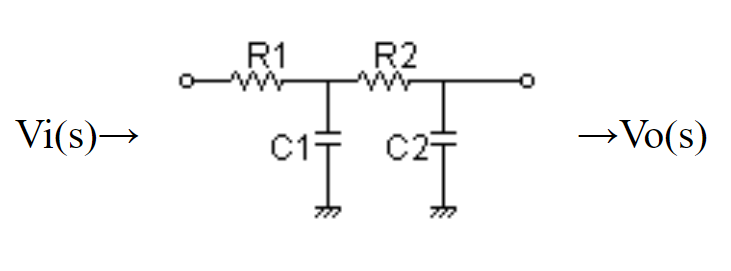
\includegraphics[width=0.5\linewidth]{Hardware/RCfilter}
	\caption{Passivt 2. Ordens lavpasfilter - RC}
	\label{fig:RCfilter}
\end{figure}

Efter beregninger på RC-filteret, se afsnit \vref{RC-filter}, vurderes det, at det er bedre for systemet med et aktivt filter. Vores endelige beslutning omkring filtertype falder derfor på et aktivt 2. ordens lavpasfilter af typen Sallen Key.

\textbf{Sallen Key filter:} 

\begin{figure}[h!]
	\centering
	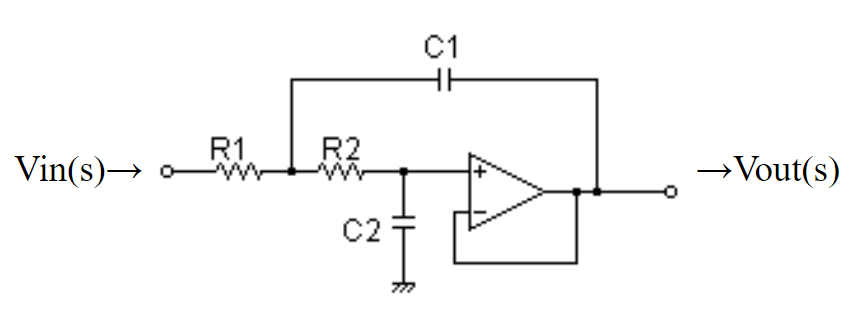
\includegraphics[width=0.5\linewidth]{Hardware/SallenKey}
	\caption{Aktivt 2. Ordens lavpasfilter - Sallen Key}
	\label{fig:SallenKey}
\end{figure}

\clearpage
  
\subsection{Beregninger: RC-filter} \label{RC-filter}
\vspace{0.2 cm}
Overføringsfunktion: 
\[ T(s)=K \cdot \frac{\omega_{0}^{2}}{{s^{2}+2 \cdot \zeta \cdot \omega_{0}\cdot s+\omega_{0}^{2}}} \]

Gain:
\[ K=1 \]



Da vi ikke forstærker signalet yderligere med dette filter sættes $K=1$.
\[ V_{in}=4V \]
\[ V_{out}=4V \]

Frekvens:
\[ \omega_{0}=\frac{1}{\sqrt{R_{1} \cdot R_{2} \cdot C_{1} \cdot C_{2}}} \]

Dæmpningsfaktor:
\[ \zeta= \frac{R_{1} \cdot C_{1} + R_{1} \cdot C_{2}+R_{2} \cdot C_{2}}{2 \cdot \sqrt{R_{1} \cdot R_{2} \cdot C_{1} \cdot C_{2}}} \]

Frekvens og dæmpningsfaktor indsættes nu i overføringsfunktionen:
\[ T(s)=\frac{\omega_{0}=\frac{1}{R_{1} \cdot R_{2} \cdot C_{1} \cdot C_{2}}}{s^{2}+2 \cdot (\frac{R_{1} \cdot C_{1} + R_{1} \cdot C_{2}+R_{2} \cdot C_{2}}{2 \cdot \sqrt{R_{1} \cdot R_{2} \cdot C_{1} \cdot C_{2}}}) \cdot (\frac{1}{\sqrt{R_{1} \cdot R_{2} \cdot C_{1} \cdot C_{2}}}) \cdot s + (\frac{1}{R_{1} \cdot R_{2} \cdot C_{1} \cdot C_{2}})}  \]

$T(s)$ simplificeres:
\[ T(s)=\frac{1}{s \cdot C_{1} \cdot R_{1} +s \cdot C_{2} \cdot R_{1}+s \cdot C_{2} \cdot R_{2}+s^{2}\cdot C_{1} \cdot C_{2} \cdot R_{1} \cdot R_{2} +1} \]

$T(s)$ simplificeres yderligere:
\[ T(s)=\frac{1}{(R_{1} \cdot C_{1} \cdot s+1) \cdot (R_{2} \cdot C_{2} \cdot s +1) \cdot R_{1} \cdot C_{2} \cdot s} \]

For at gøre beregningen af komponenterne mulig bestemmes $ C_{1} $ og $ C_{2} $ med samme værdi. Værdien er valgt tilfældigt ud fra hvilke komponenter, der findes i laboratoriet:
\[ C_{1} = 220 \cdot 10^{-9} \]
\[ C_{2} = 220 \cdot 10^{-9} \]


\subsection{Beregninger: Sallen Key filter}

\subsection{Test af filter}
\vspace{0.5 cm}
\begin{table}[h!]
	\begin{tabular}{l|l|l|l|l}
		\multicolumn{5}{l}{\textbf{Test af filter}} \\
		\hline
		\textbf{Frekvens (Hz)} & \textbf{Amplitude (V)} & \textbf{Offset} & \textbf{Amplitude (V)} & \textbf{dB} \\
		& Input &  & Output & (20*log(Vout/Vin) \\
		\hline
		10 & 2 & 0 & 2 & 0 \\
		\hline
		30 & 2 & 0 & 1,905 & -0,422700313 \\
		\hline
		40 & 2 & 0 & 1,7164 & -1,328229796 \\
		\hline
		50 & 2 & 0 & 1,4416 & -2,843704441 \\
		\hline
		60 & 2 & 0 & 1,1668 & -4,680671504 \\
		\hline
		70 & 2 & 0 & 0,9577 & -6,396010165 \\
		\hline
		80 & 2 & 0 & 0,7546 & -8,466263896 \\
		\hline
		90 & 2 & 0 & 0,6172 & -10,21208157 \\
		\hline
		100 & 2 & 0 & 0,5037 & -11,9771609 \\
		\hline
		110 & 2 & 0 & 0,432 & -13,31092498 \\
		\hline
		120 & 2 & 0 & 0,3603 & -14,88731467 \\
		\hline
		130 & 2 & 0 & 0,3066 & -16,2891569 \\
		\hline
		140 & 2 & 0 & 0,2707 & -17,3708348 \\
		\hline
		150 & 2 & 0 & 0,2286 & -18,83907539 \\
		\hline
		170 & 2 & 0 & 0,1772 & -21,05132556 \\
		\hline
		190 & 2 & 0 & 0,1438 & -22,86542219 \\
		\hline
		210 & 2 & 0 & 0,1163 & -24,70900562 \\
		\hline
		250 & 2 & 0 & 0,084 & -27,53501419 \\
		\hline
		290 & 2 & 0 & 0,0613 & -30,27139042 \\
		\hline
		330 & 2 & 0 & 0,0467 & -32,6342623 \\
		\hline
		370 & 2 & 0 & 0,0374 & -34,56316787 \\
		\hline
		410 & 2 & 0 & 0,0299 & -36,50717615 \\
		\hline
		450 & 2 & 0 & 0,0247 & -38,16666085 \\
		\hline
		500 & 2 & 0 & 0,0201 & -39,95667876
	\end{tabular}
\end{table}